\subsection*{2.1}
  % Implement the CE-CC amplifier shown below:
    \begin{figure}[h!]
        \centering
        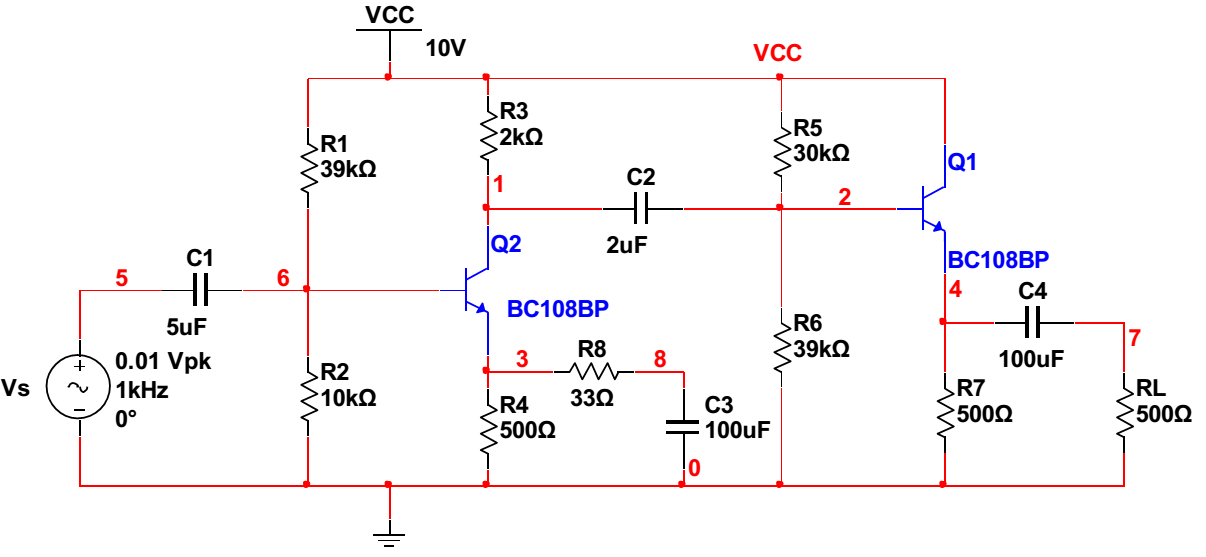
\includegraphics[width=13cm]{fig2-1.png}
        \captionof{figure}{The CE-CC amplifier to be implemented in Task 2.1}
    \end{figure}    

\subsection*{2.2}
  % Using  proper  simulation  techniques,  determine  the  following  parameters  of  the  circuit:
  \subsection*{(i) Midband voltage gain}
  \subsection*{(ii) Input resistance}
  \subsection*{(iii) Output resistance}
  \subsection*{(iv) Lower 3dB frequency}
  \subsection*{(v) Upper 3dB frequency}
  \subsection*{(vi) Output voltage when total harmonics distortion (THD) < 5\%}
  In order to evaluate the THD in the circuit, a fourier analysis has to be done. The input voltage is lowered gradually from 0.01 V until the THD is lower than 5\%. When that value was reached for the THD the Output voltage was determined 2.5471 V and the input voltage was then at 0.0731 V.
  \begin{figure}[h!]
        \centering
        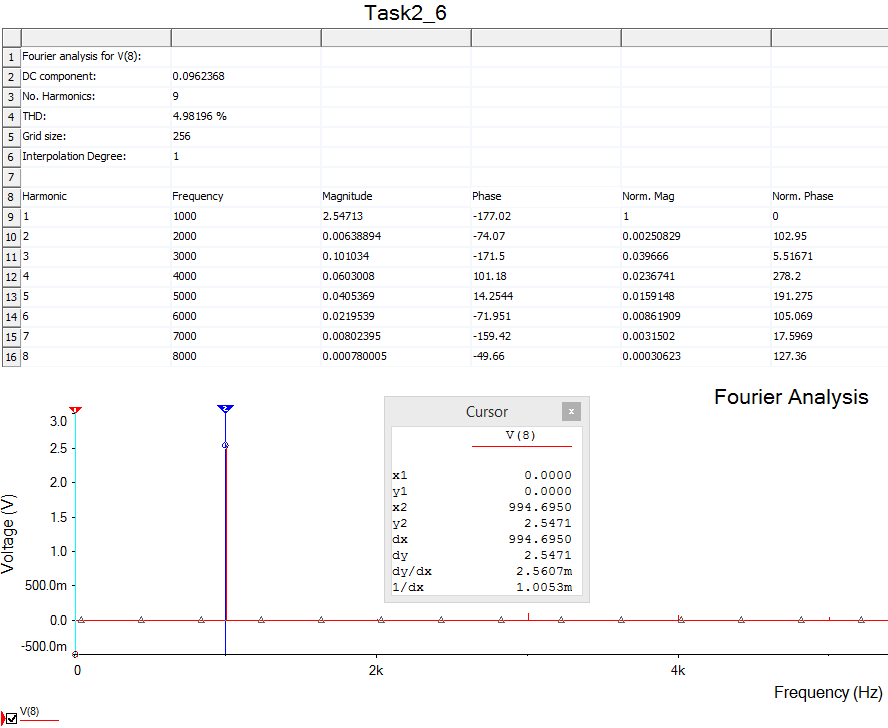
\includegraphics[width=16cm]{Task2_6_MaxOutPutVoltage.png}
        \captionof{figure}{The fourier analysis with THD $\approx$ 5\%}
    \end{figure}
    
\pagebreak
  
\subsection*{2.3}
  % Summarize  the  circuit  parameters  in  a  table  and  attach  relevant  plots.  Explain  the
  % simulation techniques that you exploited.
  